% Provenance (never printed): see sources/outline_sources.md (Year 3: gravitational
% potential, spherical harmonics, J2, reference ellipsoid, geoid, satellite gravimetry,
% flexure of the lithosphere). Brief: sources/book5/BRIEFS.md, ch. 3. Curves from
% figdata/bachelor-3/hydrostatic_figure.py, ice_mass.py (IMBIE 2021), flexure.py.
% Exercise and problem values in the Book 5 scratch calculator calc/ch03.py.
\chapter{Gravity and the Figure of the Earth}\label{ch:b3:gravity-geodesy}

Two satellites fly one behind the other round the Earth, at an altitude of more
than \qty{500}{km} and about \qty{220}{km} apart, and measure the distance
between them all the time, to within a micrometre.
% ledger: geod5:grace, geod5:grace-ranging
When they pass over a place where mass is concentrated, the leading satellite
is pulled ahead first and the gap opens; then the trailing one is pulled in
turn and the gap closes. From those tiny changes, month after month since 2002,
the Earth's gravity field has been mapped as it changes: the water stored in
river basins rises and falls with the seasons, and the great ice sheets of
Greenland and Antarctica lose mass year after year. Gravity weighs what the eye
cannot see. This chapter builds the gravity field of a rotating planet from its
potential, finds in it the flattening and the moment of inertia, follows its
anomalies up to orbit, and then turns to one of the things gravity reveals at
the surface: the bending of the lithosphere under the weight of a volcano.

\begin{recall}
Newton's law of gravitation, the gravitational potential energy and the
centrifugal force in a rotating frame are the physics books'; the moments of
inertia of a solid and the Legendre polynomials $P_2(x) = (3x^2 - 1)/2$ are in
the physics and mathematics books' university volumes, Young's modulus $E$ and
Poisson's ratio $\nu$ in the physics books' Year 3 volume. Geodesy and the
flattening $f = (a - b)/a$ of an ellipsoid of semi-axes $a > b$ were met in
grade 10. Isostasy, Airy compensation, normal gravity, the geoid, the geoid
height and the gravity anomalies were defined in the Year 1 volume, in its
chapter on isostasy and gravity anomalies.
\end{recall}

\section{The geopotential}

On a rotating planet a body at rest feels the attraction of the planet's mass
and, in the frame that turns with it, the centrifugal force. Both derive from a
potential.

\begin{definition}[Geopotential]\label{def:b3:gravity-geodesy:geopotential}
The \emph{geopotential}\index{geopotential} is the potential energy per unit
mass, in the frame rotating with the Earth at the angular velocity $\omega$, of
gravitation and the centrifugal force together:
\[
  W(\mathbf r) = V(\mathbf r) + \Phi(\mathbf r),\qquad
  V(\mathbf r) = -G\int_{\text{Earth}}\frac{\mathrm dm'}{|\mathbf r - \mathbf r'|},\qquad
  \Phi(\mathbf r) = -\tfrac12\omega^2 s^2,
\]
where $s$ is the distance from the rotation axis. Gravity is
$\mathbf g = -\nabla W$, and the surfaces $W = \text{const}$ are its level
surfaces: gravity is everywhere normal to them.
\end{definition}

A plumb line hangs along $-\nabla W$, and still water settles on a level
surface. A rotating fluid planet therefore takes the shape of one of its own
level surfaces: the centrifugal potential, deepest at the equator, swells the
equator and flattens the poles.

\begin{omfigure}
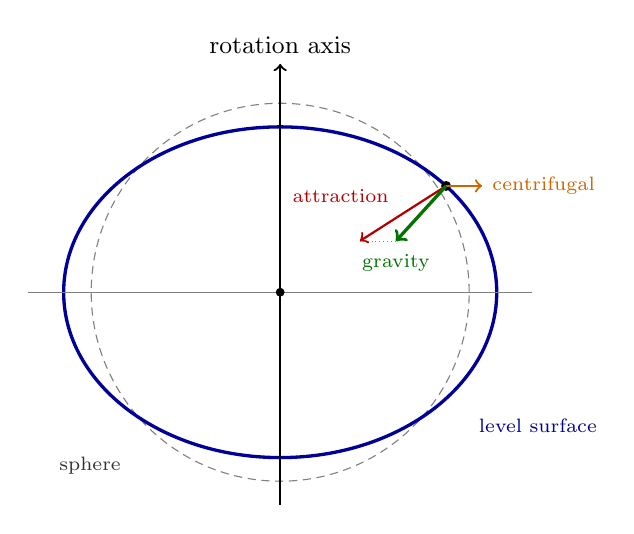
\begin{tikzpicture}[font=\small, x=1cm, y=1cm]
\draw[gray, densely dashed] (0,0) circle (2.4);
\draw[very thick, blue!60!black] (0,0) ellipse (2.75 and 2.1);
\draw[->, thick] (0,-2.7) -- (0,2.9) node[above] {rotation axis};
\draw[gray] (-3.2,0) -- (3.2,0);
\fill (0,0) circle (1.6pt);
% a point at latitude 40 deg (parameter) on the ellipse; the attraction points at
% the centre, the centrifugal force is horizontal, and their sum is drawn along the
% inward normal of the ellipse: lengths solved so that the sum is normal (calc/ch03_fig.py)
\coordinate (P) at (2.107,1.350);
\fill (P) circle (1.8pt);
\draw[->, thick, red!70!black] (P) -- (1.012,0.650);
\node[font=\scriptsize, red!70!black, anchor=south east] at (1.50,1.02) {attraction};
\draw[->, thick, orange!80!black] (P) -- (2.565,1.350) node[right, font=\scriptsize] {centrifugal};
\draw[gray, densely dotted] (1.012,0.650) -- (1.470,0.650);
\draw[->, very thick, green!45!black] (P) -- (1.470,0.650);
\node[font=\scriptsize, green!45!black, anchor=north] at (1.470,0.600) {gravity};
\node[blue!60!black, anchor=west, font=\scriptsize] at (2.4,-1.7) {level surface};
\node[gray!40!black, anchor=east, font=\scriptsize] at (-1.9,-2.2) {sphere};
\end{tikzpicture}

\par\smallskip{\small A level surface of a rotating planet (schematic, the
flattening greatly exaggerated). At each point, gravity, the sum of the
attraction and the centrifugal force, is normal to the level surface; it does
not point at the centre, except at the poles and on the equator.}
\label{fig:b3:gravity-geodesy:equipotential}
\end{omfigure}

Outside the planet the gravitational potential obeys Laplace's equation, and
its solutions regular at infinity are the solid spherical harmonics.

\begin{proposition}[Spherical-harmonic expansion of the geopotential]\label{prop:b3:gravity-geodesy:harmonics}
Outside a body of mass $M$ and equatorial radius $a$, with the origin at its
centre of mass and the $z$ axis along its axis of rotation, the gravitational
potential at the distance $r$, colatitude $\theta$ and longitude $\lambda$ is
\begin{multline*}
  V = -\frac{GM}{r}\Biggl[1 - \sum_{n=2}^{\infty}\left(\frac ar\right)^nJ_nP_n(\cos\theta)\\
  + \sum_{n=2}^{\infty}\sum_{m=1}^{n}\left(\frac ar\right)^nP_{nm}(\cos\theta)
  (C_{nm}\cos m\lambda + S_{nm}\sin m\lambda)\Biggr],
\end{multline*}
with the Legendre polynomials $P_n$ and the associated functions $P_{nm}$; the
coefficients $J_n$, $C_{nm}$, $S_{nm}$ are numbers, fitted to observations. For
a body symmetric about its axis, only the zonal terms $J_n$ remain. No term of
degree 1 appears.
\end{proposition}

\begin{proof}
The separation of variables of Laplace's equation in spherical coordinates
gives the regular-at-infinity solutions $r^{-(n+1)}P_{nm}(\cos\theta)e^{\pm
im\lambda}$ (the mathematics books' university volumes); any potential outside
the masses is a sum of them. The term of degree 0 is $-GM/r$, the potential of
the whole mass. The degree-1 terms are proportional to the first moments
$\int\mathbf r'\,\mathrm dm'$, which vanish when the origin is the centre of
mass. Axial symmetry removes every term that depends on $\lambda$.
\end{proof}

\begin{definition}[Dynamical form factor]\label{def:b3:gravity-geodesy:j2}
The \emph{dynamical form factor}\index{dynamical form factor} $J_2$ of a planet
is the coefficient of its degree-2 zonal harmonic: the largest departure of its
external potential from that of a sphere, caused by its oblateness. For the
Earth, $J_2 = \num{1.08263e-3}$.
% ledger: geod5:grs80-defining
\end{definition}

\begin{theorem}[MacCullagh's formula]\label{thm:b3:gravity-geodesy:maccullagh}
Let $A$, $B$, $C$ be the principal moments of inertia of a body of mass $M$
about axes through its centre of mass, and $I$ its moment of inertia about the
line from the centre of mass to an external point at the distance $r$. To order
$r^{-3}$ the gravitational potential at that point is given by
\emph{MacCullagh's formula}\index{MacCullagh's formula}
\[
  V = -\frac{GM}{r} - \frac{G(A + B + C - 3I)}{2r^3} .
\]
For a body symmetric about the $z$ axis ($A = B$),
$V = -\dfrac{GM}{r} + \dfrac{G(C - A)}{r^3}P_2(\cos\theta)$, so that
\[
  J_2 = \frac{C - A}{Ma^2} .
\]
\end{theorem}

\begin{proof}
With $\hat{\mathbf r}$ the unit vector towards the point and $r' \ll r$,
\[
  \frac{1}{|\mathbf r - \mathbf r'|} = \frac1r + \frac{\hat{\mathbf r}\cdot\mathbf r'}{r^2}
  + \frac{3(\hat{\mathbf r}\cdot\mathbf r')^2 - r'^2}{2r^3} + O(r^{-4}).
\]
Integrated over the mass, the first term gives $M/r$ and the second vanishes
(centre of mass). For the third, $\int r'^2\,\mathrm dm' = (A + B + C)/2$, since
$A + B + C = \int 2r'^2\,\mathrm dm'$, and $\int(\hat{\mathbf r}\cdot\mathbf
r')^2\,\mathrm dm' = \int r'^2\,\mathrm dm' - I$, the square of the distance to
the line being $r'^2 - (\hat{\mathbf r}\cdot\mathbf r')^2$. The bracket integrates
to $3(A + B + C)/2 - 3I - (A + B + C)/2 = A + B + C - 3I$. For $A = B$, the
moment about a line at colatitude $\theta$ is $I = A\sin^2\theta + C\cos^2\theta$,
and $2A + C - 3I = (C - A)(1 - 3\cos^2\theta) = -2(C - A)P_2(\cos\theta)$.
Comparing with \cref{prop:b3:gravity-geodesy:harmonics} gives
$J_2Ma^2 = C - A$.
\end{proof}

The degree-2 term of the potential therefore measures the difference of the
moments of inertia, not the moments themselves. The precession of the Earth's
axis, driven by the torques of the Sun and Moon on the equatorial bulge,
measures the dynamical ellipticity $H = (C - A)/C$; together, $J_2$ and $H$ give
$C/(Ma^2)$, the moment-of-inertia factor, \num{0.3308} for the Earth,
% ledger: earth:MoI
well below the \num{0.4} of a uniform sphere: the mass is concentrated towards
the centre.

\section{The rotating ellipsoid}

\begin{definition}[Reference ellipsoid]\label{def:b3:gravity-geodesy:ellipsoid}
A \emph{reference ellipsoid}\index{reference ellipsoid} is an ellipsoid of
revolution, of equatorial semi-axis $a$ and flattening $f$, chosen so that it
is itself a level surface of a model potential: the potential of a rotating
body of mass $M$ with the angular velocity $\omega$ and the \omterm{def:b3:gravity-geodesy:j2}{dynamical form
factor} $J_2$ of the Earth. Four constants define it; the Geodetic Reference
System 1980 takes
\begin{gather*}
  a = \qty{6378137}{m},\qquad GM = \qty{3.986005e14}{m^3.s^{-2}},\\
  J_2 = \num{1.08263e-3},\qquad \omega = \qty{7.292115e-5}{rad.s^{-1}},
\end{gather*}
and derives from them the flattening $f = \num{0.00335281068}$
($1/f = \num{298.257222}$) and the semi-minor axis
$b = \qty{6356752.3141}{m}$.
% ledger: geod5:grs80-defining, geod5:grs80-derived
\end{definition}

The potential of the model, the normal potential, is known in closed form, and
so is its gravity on the ellipsoid, the normal gravity of the Year 1 volume.

\begin{proposition}[Somigliana's formula]\label{prop:b3:gravity-geodesy:somigliana}
On a \omterm{def:b3:gravity-geodesy:ellipsoid}{reference ellipsoid} with semi-axes $a$, $b$ and normal gravity
$\gamma_e$ at the equator and $\gamma_p$ at the poles, normal gravity at the
geodetic latitude $\varphi$ is given by \emph{Somigliana's
formula}\index{Somigliana's formula}
\[
  \gamma(\varphi) = \frac{a\gamma_e\cos^2\varphi + b\gamma_p\sin^2\varphi}
  {\sqrt{a^2\cos^2\varphi + b^2\sin^2\varphi}} .
\]
For the Geodetic Reference System 1980, $\gamma_e = \qty{9.7803267715}{m.s^{-2}}$
and $\gamma_p = \qty{9.8321863685}{m.s^{-2}}$, and the series
$\gamma = 9.780327(1 + 0.0053024\sin^2\varphi - 0.0000058\sin^22\varphi)$
\unit{m.s^{-2}} reproduces the formula to \qty{0.1}{\milli\gal}.
% ledger: geod5:grs80-derived, moritz:grs80 (Book 3, read-only)
\end{proposition}
\admitted

How flat should a rotating planet be? If it is a fluid in hydrostatic
equilibrium, its flattening is fixed by its rotation and by how its mass is
distributed in depth.

\begin{proposition}[Clairaut and Darwin--Radau relations]\label{prop:b3:gravity-geodesy:clairaut}
For a planet in hydrostatic equilibrium, with $m = \omega^2a^2b/(GM)$ the ratio
of the centrifugal to the gravitational acceleration at the equator, to first
order in $f$ and $m$:
\[
  J_2 = \frac{2f - m}{3}\qquad\text{(Clairaut)},\qquad
  \frac{C}{Ma^2} = \frac23\left[1 - \frac25\sqrt{\frac52\frac mf - 1}\right]
  \qquad\text{(Darwin--Radau)} .
\]
A uniform planet ($C/Ma^2 = 0.4$) has $f = 5m/4$; a planet whose mass is
concentrated towards the centre is less flattened.
\end{proposition}
\admitted

The Clairaut relation, with the Earth's $m = \num{0.00344979}$, turns its
measured $J_2$ into $f = \num{0.0033488}$, or $1/298.6$: within
\qty{0.12}{\percent} of the flattening of the ellipsoid. The Darwin--Radau
relation, with the moment-of-inertia factor, gives the flattening the Earth
would have if it were a fluid in equilibrium: $1/299.9$, against the measured
$1/298.26$. The Earth is a little flatter than a fluid planet with its rotation
and its mass distribution would be: its equatorial bulge stands about
\qty{116}{m} higher than hydrostatic equilibrium predicts. The Earth is not
exactly a fluid in equilibrium, and the small difference is itself a
measurement of the stresses its interior sustains.

\begin{omfigure}
\begin{tikzpicture}
\begin{axis}[omrecord, width=0.74\linewidth, height=0.44\linewidth,
  xmin=0.3, xmax=0.4, ymin=225, ymax=340,
  xlabel={moment-of-inertia factor $C/(Ma^2)$}, ylabel={hydrostatic $1/f$},
  xtick={0.30,0.32,0.34,0.36,0.38,0.40},
  xticklabel style={/pgf/number format/fixed, /pgf/number format/precision=2}]
\addplot[blue!70!black, thick] table[x=moi, y=f_inv] {figdata/out/bachelor-3-hydrostatic_figure-curve.dat};
\draw[gray, densely dashed] (axis cs:0.3308,225) -- (axis cs:0.3308,299.88);
\draw[gray, densely dashed] (axis cs:0.3,299.88) -- (axis cs:0.3308,299.88);
\fill[blue!70!black] (axis cs:0.3308,299.88) circle (2pt);
\node[font=\scriptsize, anchor=south west] at (axis cs:0.3315,301) {hydrostatic Earth, $1/f = 299.9$};
\draw[red!70!black, thick] (axis cs:0.3,298.26) -- (axis cs:0.4,298.26);
\node[font=\scriptsize, anchor=north east, red!70!black] at (axis cs:0.399,296.5) {observed, $1/f = 298.26$};
\fill (axis cs:0.4,231.9) circle (2pt);
\node[font=\scriptsize, anchor=east] at (axis cs:0.397,233) {uniform planet};
\end{axis}
\end{tikzpicture}

\par\smallskip{\small The flattening of a fluid planet with the Earth's rotation,
against its moment-of-inertia factor, from the Darwin--Radau relation
(computed from the Geodetic Reference System 1980). The more the mass is
concentrated towards the centre, the rounder the planet. At the Earth's
\num{0.3308} the hydrostatic flattening is $1/299.9$, a little less than the
observed $1/298.26$.}
\label{fig:b3:gravity-geodesy:hydrostatic}
\end{omfigure}

\section{The geoid and the disturbing potential}

The geoid is the level surface of the real \omterm{def:b3:gravity-geodesy:geopotential}{geopotential} that coincides with
mean sea level; the \omterm{def:b3:gravity-geodesy:ellipsoid}{reference ellipsoid} is a level surface of the normal
potential $U$ with the same value, $U_0 = W_0$. Their separation, the geoid
height $N$, is set by the difference of the two potentials.

\begin{proposition}[Bruns' formula]\label{prop:b3:gravity-geodesy:bruns}
Let $T = W - U$ be the disturbing potential. The geoid height at a point is
given by \emph{Bruns' formula}\index{Bruns' formula}
\[
  N = -\frac{T}{\gamma},
\]
where $T$ is evaluated on the geoid and $\gamma$ is normal gravity there. A
mass excess, which deepens the potential ($T < 0$), raises the geoid.
\end{proposition}

\begin{proof}
Let P be on the geoid and Q the point of the ellipsoid below it, at the distance
$N$. Since $U$ increases outwards at the rate $\gamma$,
$U(\mathrm P) = U(\mathrm Q) + \gamma N = U_0 + \gamma N$. Then
$W_0 = W(\mathrm P) = U(\mathrm P) + T(\mathrm P) = U_0 + \gamma N + T$, and
$W_0 = U_0$ gives $N = -T/\gamma$.
\end{proof}

A geoid height of \qty{50}{m} is a potential difference of only
\qty{490}{J.kg^{-1}}, one part in \num{e5} of the \omterm{def:b3:gravity-geodesy:geopotential}{geopotential}. The geoid
heights of the Earth range from about $+\qty{85}{m}$ at Iceland to
$-\qty{106}{m}$ in southern India,
% ledger: nasa:geoid-range (Book 3, read-only)
a range of under \qty{200}{m} on a planet whose equatorial and polar radii
differ by \qty{21}{km}.

\section{Satellite gravimetry}

\begin{definition}[Satellite gravimetry]\label{def:b3:gravity-geodesy:satgrav}
\emph{Satellite gravimetry}\index{satellite gravimetry} determines the Earth's
gravity field from the motion of satellites: from the long-term perturbations
of their orbits, from the changing distance between two satellites on the same
orbit, or from gradiometers that measure the differences of gravity across the
spacecraft.
\end{definition}

The largest perturbation of a near-Earth orbit comes from $J_2$. The
equatorial bulge exerts a torque on the inclined orbit, which turns slowly
about the Earth's axis.

\begin{proposition}[Nodal precession]\label{prop:b3:gravity-geodesy:nodal}
To first order in $J_2$, the line of nodes of a circular orbit of radius $r$ and
inclination $i$ turns at the rate
\[
  \dot\Omega = -\frac32\,nJ_2\left(\frac ar\right)^2\cos i,\qquad n = \sqrt{GM/r^3} ,
\]
westward for a prograde orbit ($i < \ang{90}$), eastward for a retrograde one.
\end{proposition}

\begin{proof}
Over many revolutions the satellite acts like a ring of mass $m_s$ spread along
its orbit. The degree-2 part of the potential,
$(GMJ_2a^2/r^3)P_2(\cos\theta)$ per unit mass, averaged over a circle inclined
at $i$, involves $\langle\cos^2\theta\rangle = \tfrac12\sin^2i$, so
$\langle P_2\rangle = \tfrac34\sin^2i - \tfrac12$, and the ring's energy is
$E(i) = m_s(GMJ_2a^2/r^3)(\tfrac34\sin^2i - \tfrac12)$. The torque about the line
of nodes is $\tau = -\mathrm dE/\mathrm di = -\tfrac32m_s(GMJ_2a^2/r^3)\sin
i\cos i$. It is perpendicular to the ring's angular momentum $L = m_snr^2$, so
it turns $\mathbf L$ about the polar axis without changing its length:
$L\sin i\,\dot\Omega = \tau$. With $GM = n^2r^3$, $\dot\Omega =
-\tfrac32nJ_2(a/r)^2\cos i$.
\end{proof}

The rate is several degrees per day for a low orbit near the equator; at an
inclination a little beyond \ang{90} it matches the Sun's yearly motion, and the
orbit keeps the same orientation to the Sun all year (exercise 12). Measured on
many satellites at different inclinations, such precessions give $J_2$ and the
higher zonal harmonics.

A pair of satellites does better: the changing distance between them measures
the difference of the gravity they feel along the orbit. The GRACE pair flew from 2002 to 2017, and its
successor, GRACE Follow-On, since its launch on 22 May 2018, its microwave link
measuring the distance to within a micrometre and a laser link testing a
precision up to twenty times better.
% ledger: geod5:grace, geod5:grace-ranging
The field changes from month to month because water moves: snow and soil
moisture, groundwater, lakes, the oceans, the ice sheets.

\begin{omfigure}
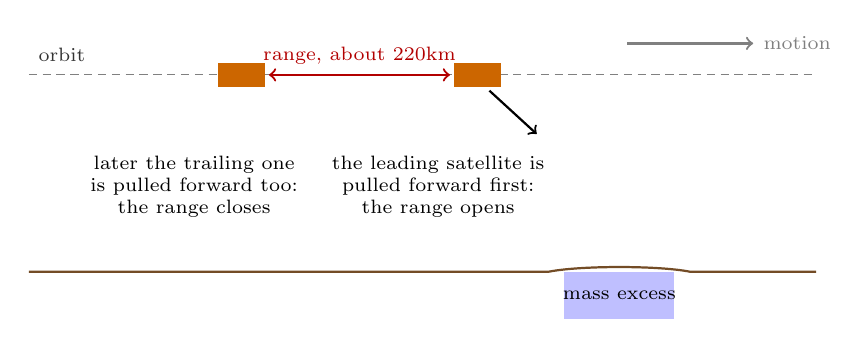
\begin{tikzpicture}[font=\small, x=1cm, y=1cm]
\draw[thick, brown!60!black] (-5,0) -- (1.6,0) .. controls (2.0,0.08) and (3.0,0.08) .. (3.4,0) -- (5,0);
\fill[blue!25] (1.8,0) rectangle (3.2,-0.6);
\node[font=\scriptsize] at (2.5,-0.3) {mass excess};
\draw[gray, densely dashed] (-5,2.5) -- (5,2.5);
\node[gray!40!black, font=\scriptsize, anchor=south west] at (-5,2.55) {orbit};
\fill[orange!80!black] (-2.6,2.35) rectangle (-2.0,2.65);
\fill[orange!80!black] (0.4,2.35) rectangle (1.0,2.65);
\draw[<->, red!70!black, thick] (-1.95,2.5) -- (0.35,2.5) node[midway, above, font=\scriptsize] {range, about \qty{220}{km}};
\draw[->, thick] (0.85,2.3) -- (1.45,1.75);
\draw[->, thick, gray] (2.6,2.9) -- (4.2,2.9) node[right, font=\scriptsize] {motion};
\node[font=\scriptsize, anchor=north, align=center] at (0.2,1.6) {the leading satellite is\\pulled forward first:\\the range opens};
\node[font=\scriptsize, anchor=north, align=center] at (-2.9,1.6) {later the trailing one\\is pulled forward too:\\the range closes};
\end{tikzpicture}

\par\smallskip{\small The principle of the satellite pair (schematic, not to
scale). Approaching a mass excess, the leading satellite feels its attraction
first and is accelerated forward, so the range between the two increases; when
the trailing satellite comes over the mass the range decreases again. The range
rate, measured continuously, is inverted for the gravity field.}
\label{fig:b3:gravity-geodesy:grace}
\end{omfigure}

\begin{omfigure}
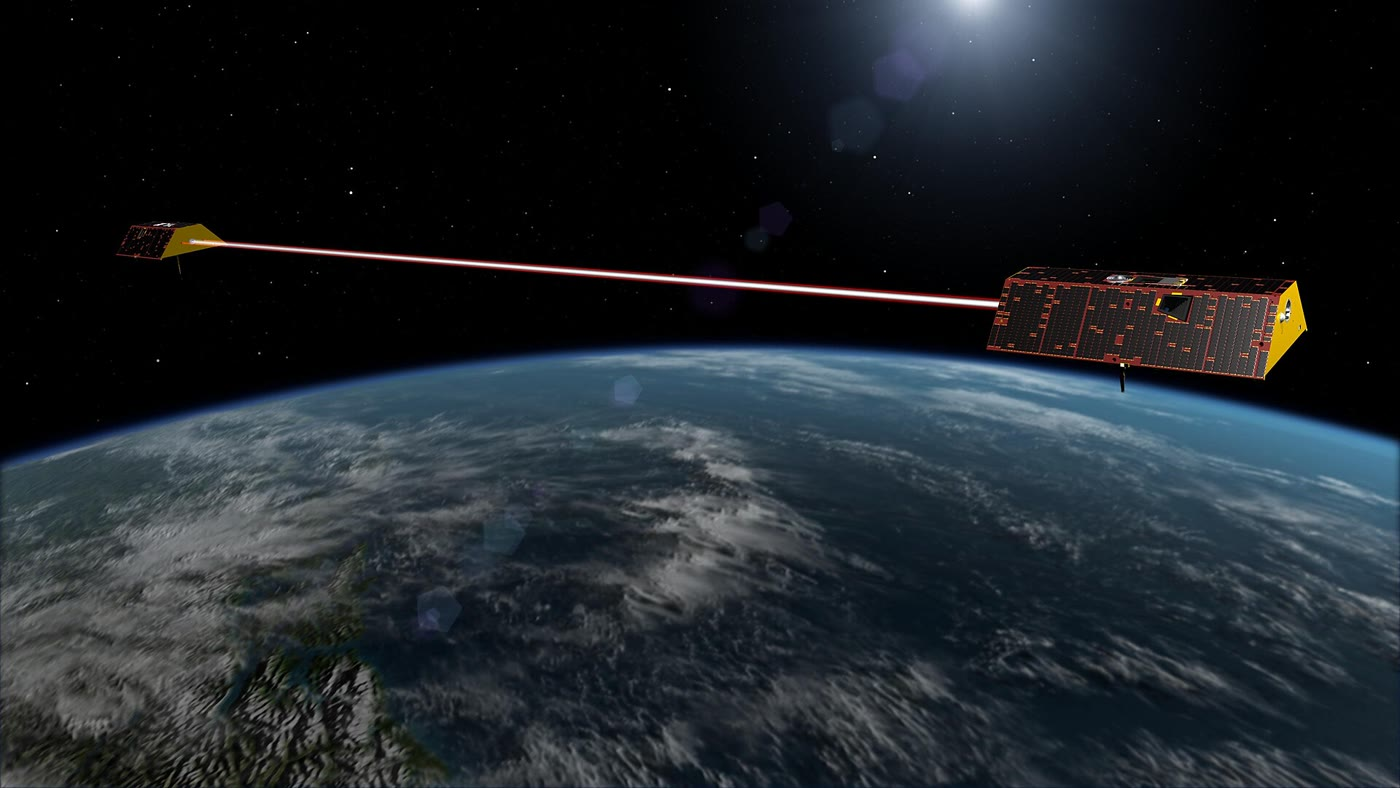
\includegraphics[width=0.66\linewidth]{images/book5/b3-grace-fo-concept.jpg}

\par\smallskip{\small The two GRACE Follow-On satellites, an artist's view (the
distance between them is greatly shortened). The red beam stands for the laser
ranging link. NASA/JPL-Caltech, public domain.}
\label{fig:b3:gravity-geodesy:grace-photo}
\end{omfigure}

\begin{definition}[Equivalent water height]\label{def:b3:gravity-geodesy:ewh}
A change of the gravity field that varies slowly over distances much larger
than the thickness of the layer where the mass moved can be represented by a
change of surface density $\sigma$ (\unit{kg.m^{-2}}) on a thin shell at the
Earth's surface. The \emph{equivalent water height}\index{equivalent water height}
is the thickness of fresh water with the same surface density:
\[
  h_w = \frac{\sigma}{\rho_w} .
\]
\end{definition}

A metre of water over a basin of \qty{1e6}{km^2} is \qty{1e15}{kg}, or
\qty{1000}{Gt}. Sea level is the other side of the ledger: \qty{360}{Gt} of ice
added to the ocean raises it by about a millimetre.
% ledger: data:b5-imbie
\omterm{def:b3:gravity-geodesy:satgrav}{Satellite gravimetry}, satellite altimetry and the balance of snowfall against
ice discharge each measure the mass balance of the ice sheets; reconciled, they
give the series below.

\begin{omfigure}
\begin{tikzpicture}
\begin{axis}[omrecord, width=0.82\linewidth, height=0.5\linewidth,
  xmin=1992, xmax=2021, ymin=-5600, ymax=600,
  xlabel={year}, ylabel={cumulative mass change (\unit{Gt})},
  xticklabel style={/pgf/number format/1000 sep={}},
  legend pos=south west, legend cell align=left, legend style={font=\scriptsize}]
\addplot[name path=gl, draw=none, forget plot] table[x=year, y=lo] {figdata/out/bachelor-3-ice_mass-greenland.dat};
\addplot[name path=gh, draw=none, forget plot] table[x=year, y=hi] {figdata/out/bachelor-3-ice_mass-greenland.dat};
\addplot[blue!25, forget plot] fill between[of=gl and gh];
\addplot[name path=al, draw=none, forget plot] table[x=year, y=lo] {figdata/out/bachelor-3-ice_mass-antarctica.dat};
\addplot[name path=ah, draw=none, forget plot] table[x=year, y=hi] {figdata/out/bachelor-3-ice_mass-antarctica.dat};
\addplot[red!20, forget plot] fill between[of=al and ah];
\addplot[blue!70!black, thick] table[x=year, y=cum] {figdata/out/bachelor-3-ice_mass-greenland.dat};
\addlegendentry{Greenland}
\addplot[red!70!black, thick] table[x=year, y=cum] {figdata/out/bachelor-3-ice_mass-antarctica.dat};
\addlegendentry{Antarctica}
\draw[gray, densely dotted] (axis cs:2002.25,-5600) -- (axis cs:2002.25,600);
\draw[gray, densely dotted] (axis cs:2017.5,-5600) -- (axis cs:2017.5,600);
\node[font=\scriptsize, gray!40!black, anchor=north] at (axis cs:2009.9,550) {GRACE years};
\end{axis}
\end{tikzpicture}

\par\smallskip{\small Cumulative mass change of the Greenland and Antarctic ice
sheets since 1992, with one-standard-deviation bands (IMBIE 2021 reconciled
estimates from altimetry, gravimetry and the input--output method). By the end
of 2020 Greenland had lost $\num{4890} \pm \qty{460}{Gt}$ and Antarctica
$\num{2670} \pm \qty{530}{Gt}$; straight-line fits give
\qty{-176}{Gt.yr^{-1}} and \qty{-91}{Gt.yr^{-1}} over 1992--2020, and
\qty{-246}{Gt.yr^{-1}} and \qty{-127}{Gt.yr^{-1}} over the GRACE years.}
\label{fig:b3:gravity-geodesy:ice-mass}
\end{omfigure}

A gravity anomaly measured at the surface is a sum of harmonics; at the
altitude of a satellite, each is weakened by a factor that depends on its
wavelength.

\begin{proposition}[Upward continuation]\label{prop:b3:gravity-geodesy:upward}
Above the masses that cause it, a gravity anomaly that varies along the surface
as $\Delta g_0\cos kx$, with $k = 2\pi/\lambda$, is at the height $z$ (its
\emph{upward continuation}\index{upward continuation})
\[
  \Delta g(x, z) = \Delta g_0\,e^{-kz}\cos kx .
\]
\end{proposition}

\begin{proof}
Above the masses the anomalous potential, and with it the anomaly, satisfies
Laplace's equation $\partial_x^2\Delta g + \partial_z^2\Delta g = 0$. Separating
variables, $\Delta g = Z(z)\cos kx$ with $Z'' = k^2Z$, whose solution bounded as
$z \to \infty$ is $Z = \Delta g_0e^{-kz}$.
\end{proof}

At \qty{400}{km} altitude an anomaly \qty{1000}{km} long keeps \qty{8}{\percent}
of its amplitude, one \qty{100}{km} long about \num{1e-11} of it:
satellites see the long wavelengths, and surveys at the surface the short ones.

\section{Flexure of the lithosphere}

The Year 1 volume compensated a load locally, each column floating on its own.
A volcano on an oceanic plate is not compensated beneath itself alone: the
plate bends under it over a width of hundreds of kilometres, and the seafloor
around the volcano sinks into a moat, beyond which it rises in a low arch.

\begin{definition}[Lithospheric flexure, flexural rigidity, effective elastic thickness]\label{def:b3:gravity-geodesy:flexure}
\emph{Lithospheric flexure}\index{lithospheric flexure} is the bending of the
lithosphere under a load, modelled as the bending of a thin elastic plate
floating on a fluid mantle. The plate's resistance to bending is its
\emph{flexural rigidity}\index{flexural rigidity}
\[
  D = \frac{ET_e^3}{12(1 - \nu^2)},
\]
and the thickness $T_e$ of the uniform elastic plate that bends like the real
lithosphere is its \emph{effective elastic thickness}\index{effective elastic thickness}.
\end{definition}

\begin{theorem}[Flexure of a thin plate]\label{thm:b3:gravity-geodesy:plate}
A thin elastic plate of rigidity $D$, bent along one direction by a load $q(x)$
per unit area, deflected downward by $w(x)$ and floating on a mantle of density
$\rho_m$, the hollow being filled with material of density $\rho_i$, obeys the
\emph{flexure equation}\index{flexure equation}
\[
  D\frac{\mathrm d^4w}{\mathrm dx^4} + (\rho_m - \rho_i)g\,w = q(x) .
\]
\end{theorem}

\begin{proof}
In a bent plate, the fibres above the mid-plane are shortened and those below
stretched, in proportion to the curvature $w''$; integrating the bending
stress over the thickness gives the bending moment $M = -Dw''$, with the
rigidity of the definition (the plate cannot expand sideways, hence the factor
$1 - \nu^2$; the physics books' Year 3 volume). A slice $\mathrm dx$ of the plate
carries the shear force $V$ on its faces and the moment $M$. Vertical balance:
the load $q\,\mathrm dx$ downward and the buoyancy of the displaced mantle
$(\rho_m - \rho_i)gw\,\mathrm dx$ upward give $\mathrm dV/\mathrm dx = -q +
(\rho_m - \rho_i)gw$. Balance of moments gives $\mathrm dM/\mathrm dx = V$.
Then $-Dw'''' = M'' = V' = -q + (\rho_m - \rho_i)gw$.
\end{proof}

\begin{definition}[Flexural parameter, forebulge]\label{def:b3:gravity-geodesy:alpha}
The \emph{flexural parameter}\index{flexural parameter} of a plate is the
length
\[
  \alpha = \left(\frac{4D}{(\rho_m - \rho_i)g}\right)^{1/4},
\]
which sets the horizontal scale of its flexure. The \emph{forebulge}\index{forebulge}
is the low arch of upward flexure that a bent plate raises beyond the moat or
basin next to its load.
\end{definition}

\begin{proposition}[Line load on a continuous plate]\label{prop:b3:gravity-geodesy:line}
A line load $V_0$ per unit length along $x = 0$ deflects the plate by
\[
  w(x) = w_0e^{-|x|/\alpha}\left(\cos\frac{|x|}{\alpha} + \sin\frac{|x|}{\alpha}\right),
  \qquad w_0 = \frac{V_0\alpha^3}{8D} .
\]
The deflection vanishes at $|x| = 3\pi\alpha/4$, the edge of the moat; the
\omterm{def:b3:gravity-geodesy:alpha}{forebulge} crest is at $|x| = \pi\alpha$, with the height $w_0e^{-\pi} =
\num{0.0432}\,w_0$. The buoyancy of the whole deflection balances the load:
$\int(\rho_m - \rho_i)gw\,\mathrm dx = V_0$.
\end{proposition}

\begin{proof}
For $x > 0$ the equation is $w'''' + 4w/\alpha^4 = 0$; the roots of
$r^4 = -4/\alpha^4$ are $(\pm1 \pm i)/\alpha$, and the solutions that vanish far
away are $e^{-x/\alpha}(A\cos(x/\alpha) + B\sin(x/\alpha))$. Symmetry imposes
$w'(0) = 0$, which gives $A = B = w_0$. Integrating the vertical balance across
the load, the shear force $V = -Dw'''$ jumps by $-V_0$; by symmetry
$w'''(0^-) = -w'''(0^+)$, and $w'''(0^+) = 4w_0/\alpha^3$, so $8Dw_0/\alpha^3 =
V_0$. The deflection vanishes where $\tan(x/\alpha) =
-1$, first at $x = 3\pi\alpha/4$; its derivative,
$-(2w_0/\alpha)e^{-x/\alpha}\sin(x/\alpha)$, vanishes next at $x = \pi\alpha$.
Finally $\int_0^\infty e^{-u}(\cos u + \sin u)\,\mathrm du = 1$, so
$\int w\,\mathrm dx = 2w_0\alpha = V_0\alpha^4/(4D) = V_0/((\rho_m - \rho_i)g)$.
\end{proof}

\begin{proposition}[Broken plate]\label{prop:b3:gravity-geodesy:broken}
A plate broken at $x = 0$ and pushed down at its free end, as at a deep-sea
trench, deflects as $w = w_0e^{-x/\alpha}\cos(x/\alpha)$ for $x \ge 0$: the
deflection vanishes at $x = \pi\alpha/2$, and the crest of the \omterm{def:b3:gravity-geodesy:alpha}{forebulge}, the
outer rise, is at $x = 3\pi\alpha/4$, with the height $w_0e^{-3\pi/4}/\sqrt2 =
\num{0.067}\,w_0$.
\end{proposition}

\begin{proof}
The same decaying solutions, now with the free end carrying no moment,
$w''(0) = 0$, which gives $B = 0$. The zero is at $\cos(x/\alpha) = 0$; the
derivative $-(w_0/\alpha)e^{-x/\alpha}(\cos + \sin)(x/\alpha)$ vanishes at
$x = 3\pi\alpha/4$, where $w = w_0e^{-3\pi/4}\cos(3\pi/4)$.
\end{proof}

Distances are thus the key to the strength of the plate: measure where the moat
ends or where the bulge crests, and $\alpha$ follows, then $D$, then $T_e$.
Since $T_e$ enters as $\alpha^{4/3}$, a fair estimate of a distance gives a good
one of the thickness.

\begin{omfigure}
\begin{tikzpicture}
\begin{groupplot}[group style={group size=1 by 2, vertical sep=1.5cm},
  width=0.82\linewidth, height=0.36\linewidth, xmin=-400, xmax=400,
  tick label style={font=\scriptsize}, label style={font=\small}, title style={font=\small}]
\nextgroupplot[title={(a) line load: the Oru ridge on plates of three thicknesses},
  ylabel={deflection (\unit{m})}, ymin=-3000, ymax=700, y filter/.expression={-y},
  legend pos=south east, legend cell align=left, legend style={font=\scriptsize}]
\addplot[red!70!black, thick] table[x=x, y=w10] {figdata/out/bachelor-3-flexure-profiles.dat};
\addlegendentry{$T_e = \qty{10}{km}$}
\addplot[blue!70!black, thick] table[x=x, y=w25] {figdata/out/bachelor-3-flexure-profiles.dat};
\addlegendentry{$T_e = \qty{25}{km}$}
\addplot[green!45!black, thick] table[x=x, y=w40] {figdata/out/bachelor-3-flexure-profiles.dat};
\addlegendentry{$T_e = \qty{40}{km}$}
\draw[gray] (axis cs:-400,0) -- (axis cs:400,0);
\draw[->, blue!70!black] (axis cs:222,330) -- (axis cs:222,90);
\node[font=\scriptsize, blue!70!black, anchor=south] at (axis cs:222,330) {forebulge, $\pi\alpha$};
\nextgroupplot[title={(b) broken plate at a trench, $T_e = \qty{25}{km}$},
  xlabel={distance from the load or the trench (\unit{km})},
  ylabel={deflection (\unit{m})}, xmin=0, xmax=400, ymin=-1100, ymax=280,
  y filter/.expression={-y}]
\addplot[blue!70!black, thick] table[x=x, y=w] {figdata/out/bachelor-3-flexure-broken.dat};
\draw[gray] (axis cs:0,0) -- (axis cs:400,0);
\draw[->] (axis cs:166.5,200) -- (axis cs:166.5,80);
\node[font=\scriptsize, anchor=west] at (axis cs:170,200) {outer rise, $3\pi\alpha/4$};
\end{groupplot}
\end{tikzpicture}

\par\smallskip{\small Flexure of an elastic plate (computed;
$E = \qty{100}{GPa}$, $\nu = 0.25$, mantle \qty{3300}{kg.m^{-3}}, water in the
moat; vertical scale greatly exaggerated). (a) Under the load of a volcanic
ridge (\qty{4.17e12}{N.m^{-1}}), a thin plate sinks deeply and narrowly, a thick
one shallowly and widely; the \omterm{def:b3:gravity-geodesy:alpha}{forebulge} moves out from \qty{112}{km} to
\qty{316}{km}. (b) A plate broken at a trench and pushed down by \qty{1}{km}:
the outer rise stands \qty{67}{m} high, \qty{167}{km} from the trench.}
\label{fig:b3:gravity-geodesy:flexure}
\end{omfigure}

\begin{definition}[Regional isostatic compensation]\label{def:b3:gravity-geodesy:regional}
\emph{Regional isostatic compensation}\index{regional isostatic compensation}
is the support of a load by the buoyancy of a deflection spread over a region
wider than the load, through the bending strength of the lithosphere; in Airy
or Pratt compensation, by contrast, each column is compensated beneath itself.
\end{definition}

Local and regional compensation balance the same total mass, but distribute it
differently: under a narrow load on a stiff plate the root is shallow and wide,
and the gravity anomaly over the load is strongly positive, flanked by negative
anomalies over the moat. Around the islands of the Hawaiian Ridge, gravity and
seismic profiles give effective elastic thicknesses of 17 to \qty{37}{km}, and
10 to \qty{20}{km} along the older seamounts of the Emperor chain, a difference
expected from the ages of the volcanoes and of the plate they loaded; the values
follow the depth of an isotherm near
\qty{350}{\degreeCelsius} in the cooling oceanic plate.
% ledger: watts25:te
The same bending, under the weight of a mountain belt, opens the foreland
basins of the Year 2 volume, in its chapter on the Alpine orogen.

\begin{omfigure}
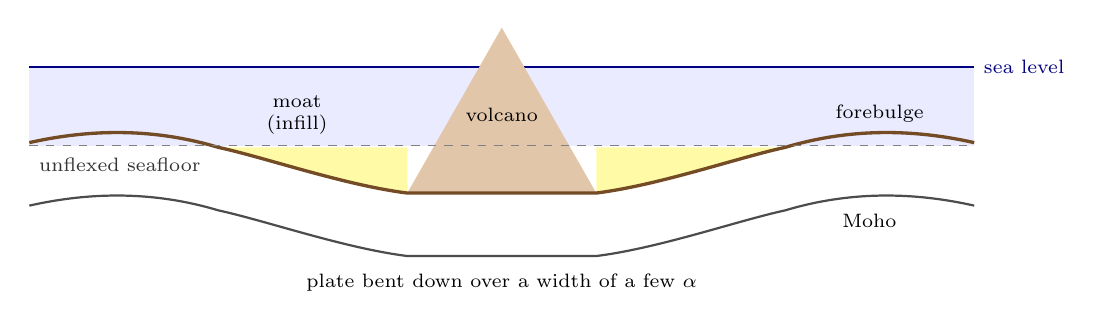
\begin{tikzpicture}[font=\scriptsize, x=1cm, y=1cm]
\fill[blue!8] (-6,0) rectangle (6,-1.0);
\draw[blue!50!black] (-6,0) -- (6,0) node[right] {sea level};
% volcano
\fill[brown!45] (-1.2,-1.6) -- (0,0.5) -- (1.2,-1.6) -- cycle;
% moat infill
\fill[yellow!35] (-1.2,-1.6) .. controls (-2.0,-1.5) and (-3.0,-1.15) .. (-3.6,-1.02) -- (-1.2,-1.02) -- cycle;
\fill[yellow!35] (1.2,-1.6) .. controls (2.0,-1.5) and (3.0,-1.15) .. (3.6,-1.02) -- (1.2,-1.02) -- cycle;
% flexed seafloor (top of crust)
\draw[very thick, brown!60!black] (-6,-0.96) .. controls (-5.2,-0.78) and (-4.4,-0.78) .. (-3.6,-1.02)
  .. controls (-3.0,-1.15) and (-2.0,-1.5) .. (-1.2,-1.6) -- (1.2,-1.6)
  .. controls (2.0,-1.5) and (3.0,-1.15) .. (3.6,-1.02) .. controls (4.4,-0.78) and (5.2,-0.78) .. (6,-0.96);
% Moho, parallel
\draw[thick, gray!60!black] (-6,-1.76) .. controls (-5.2,-1.58) and (-4.4,-1.58) .. (-3.6,-1.82)
  .. controls (-3.0,-1.95) and (-2.0,-2.3) .. (-1.2,-2.4) -- (1.2,-2.4)
  .. controls (2.0,-2.3) and (3.0,-1.95) .. (3.6,-1.82) .. controls (4.4,-1.58) and (5.2,-1.58) .. (6,-1.76);
\node[anchor=west] at (4.2,-1.95) {Moho};
\draw[dashed, gray] (-6,-1.0) -- (6,-1.0);
\node[anchor=north west, gray!40!black] at (-6,-1.03) {unflexed seafloor};
\node[anchor=south, align=center] at (-2.6,-0.98) {moat\\(infill)};
\node[anchor=south] at (4.8,-0.82) {forebulge};
\node at (0,-0.6) {volcano};
\node[anchor=north] at (0,-2.5) {plate bent down over a width of a few $\alpha$};
\end{tikzpicture}

\par\smallskip{\small A volcanic island on an oceanic plate (schematic
cross-section, vertical scale exaggerated). The plate bends under the volcano;
the hollow around it, the moat, fills with volcanic debris and sediment, and
beyond it the plate rises in a low \omterm{def:b3:gravity-geodesy:alpha}{forebulge}.}
\label{fig:b3:gravity-geodesy:moat}
\end{omfigure}

\begin{inthefield}[A relative gravity survey]
\begin{minipage}[t]{0.55\linewidth}\vspace{0pt}
An absolute gravimeter drops a corner-cube mirror in a vacuum chamber, again
and again, and times its fall with a laser interferometer and an atomic clock;
it gives gravity at one station, but it is heavy and slow to set up. The survey
itself is done with a relative gravimeter, a small spring balance that measures
differences of gravity. The geophysicist levels it on a base plate at each
station of a line, reads it, notes the time and the height, and moves on; every
few hours the loop returns to a base station, so that the slow drift of the
spring and the tides of the solid Earth can be measured and removed. A satellite
receiver on a pole nearby gives the position and the height, because gravity
changes by about \qty{0.3}{\milli\gal} for every metre of height.
\end{minipage}\hfill
\begin{minipage}[t]{0.42\linewidth}\vspace{0pt}
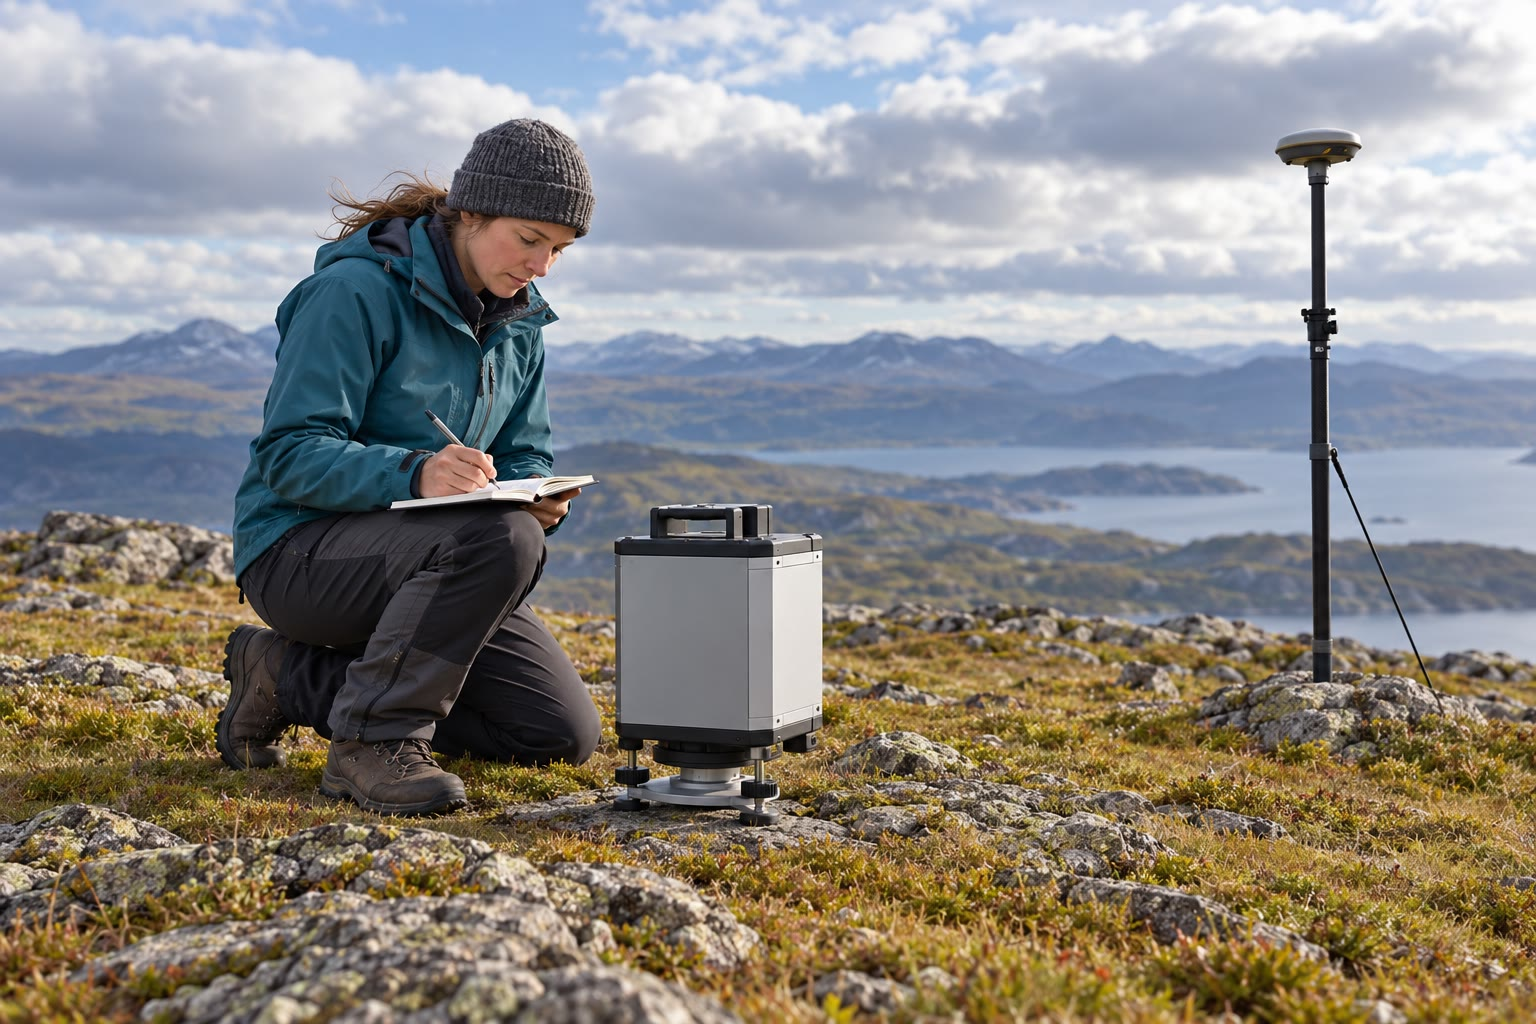
\includegraphics[width=\linewidth]{images/book5/ai/b3-gravimeter.jpg}

{\scriptsize A field gravimeter on its levelling base, with a satellite
antenna in the background (AI-generated illustration).}
\end{minipage}
\end{inthefield}

\section{Exercises}

\begin{exercise}[$\star$]\label{exo:b3:gravity-geodesy:1}
From the Geodetic Reference System 1980 values $a = \qty{6378137}{m}$ and
$f = \num{0.00335281068}$, compute the semi-minor axis $b$ and $a - b$. With
$J_2 = \num{1.08263e-3}$ and $m = \num{0.00344979}$, compute the flattening that
the Clairaut relation predicts, and compare.
\end{exercise}

\begin{exercise}[$\star$]\label{exo:b3:gravity-geodesy:2}
In a dry year, a river basin of \qty{5.0e5}{km^2} loses \qty{60}{Gt} of
water. Compute the change of \omterm{def:b3:gravity-geodesy:ewh}{equivalent water height}. By how much would the
same mass raise sea level, taking \qty{360}{Gt} per millimetre?
\end{exercise}

\begin{exercise}[$\star$]\label{exo:b3:gravity-geodesy:3}
With the series $\gamma = 9.780327(1 + 0.0053024\sin^2\varphi -
0.0000058\sin^22\varphi)$ \unit{m.s^{-2}}, compute normal gravity at the
equator, at \ang{45} and at the poles. Express the difference between the pole
and the equator in milligals.
\end{exercise}

\begin{exercise}[$\star$]\label{exo:b3:gravity-geodesy:4}
Compute the \omterm{def:b3:gravity-geodesy:flexure}{flexural rigidity} and the \omterm{def:b3:gravity-geodesy:alpha}{flexural parameter} of oceanic plates with
$T_e = \qty{10}{km}$ and $T_e = \qty{30}{km}$ ($E = \qty{100}{GPa}$,
$\nu = 0.25$, $\rho_m - \rho_w = \qty{2270}{kg.m^{-3}}$, $g =
\qty{9.81}{m.s^{-2}}$). Where are the edge of the moat and the \omterm{def:b3:gravity-geodesy:alpha}{forebulge} under a
line load?
\end{exercise}

\begin{exercise}[$\star\star$]\label{exo:b3:gravity-geodesy:5}
(a) A geoid height of $+\qty{50}{m}$: compute the disturbing potential there,
taking $\gamma = \qty{9.80}{m.s^{-2}}$. (b) Over \qty{100}{km} the geoid rises
by \qty{10}{m}. By what angle does the plumb line there differ from the normal to
the ellipsoid? Give it in seconds of arc.
\end{exercise}

\begin{exercise}[$\star\star$]\label{exo:b3:gravity-geodesy:6}
From $J_2 = \num{1.08263e-3}$ and the moment-of-inertia factor
$C/(Ma^2) = \num{0.3308}$, compute the dynamical ellipticity $H = (C - A)/C$ and
$1/H$. Which of the two numbers would a uniform Earth with the same $J_2$ change?
\end{exercise}

\begin{exercise}[$\star\star$]\label{exo:b3:gravity-geodesy:7}
A satellite flies a circular orbit \qty{500}{km} above the equatorial radius
($a = \qty{6378.137}{km}$, $GM = \qty{3.986005e14}{m^3.s^{-2}}$), inclined at
\ang{89}. Compute its period and the rate of nodal precession in degrees per day.
Why do gravity missions choose near-polar orbits?
\end{exercise}

\begin{exercise}[$\star\star$]\label{exo:b3:gravity-geodesy:8}
Two anomalies of \qty{10}{\milli\gal} at the surface have wavelengths of
\qty{100}{km} and \qty{1000}{km}. Compute their amplitudes at \qty{500}{km}
altitude.
\end{exercise}

\begin{exercise}[$\star\star$]\label{exo:b3:gravity-geodesy:9}
Seaward of a trench, the crest of the outer rise lies \qty{120}{km} from the
trench axis. Taking the broken-plate model with water above the plate, compute
$\alpha$, $D$ and $T_e$, and the distance where the plate crosses its unflexed
level.
\end{exercise}

\begin{exercise}[$\star\star\star$]\label{exo:b3:gravity-geodesy:10}
(a) Check that $w = w_0e^{-u}(\cos u + \sin u)$, $u = x/\alpha$, satisfies
$Dw'''' + (\rho_m - \rho_i)gw = 0$ for $x > 0$, with $\alpha$ as defined.
(b) Show that the bending moment $-Dw''$ is greatest under the load and changes
sign at $x = \pi\alpha/4$. (c) Where is the plate most likely to crack at its
upper surface, and why?
\end{exercise}

\begin{exercise}[$\star\star\star$]\label{exo:b3:gravity-geodesy:11}
With $m = \num{0.00344979}$ and $C/(Ma^2) = \num{0.3308}$, invert the
Darwin--Radau relation for the hydrostatic flattening. Compare with
$f = \num{0.00335281}$: compute the difference and the excess height of the
equator above the hydrostatic shape. What does it say about the mantle?
\end{exercise}

\begin{exercise}[$\star\star\star$]\label{exo:b3:gravity-geodesy:12}
A satellite on a circular orbit \qty{700}{km} high is to keep the same
orientation relative to the Sun all year: its node must advance by \ang{360} in
a tropical year of \num{365.242}~days. Compute the inclination required.
\end{exercise}

\section{Problem: The Moat around the Oru Ridge}

\begin{problem}[{Weekend problem --- the figure of the Earth, a volcanic load,
its flexural moat and what satellites see of it}]
\label{pb:b3:gravity-geodesy:1}
% values: calc/ch03.py; GRS80 (geod5:grs80-*), earth:MoI; flexure.py
Oru is an invented volcanic ridge in an ocean: a straight chain of coalesced
volcanoes \qty{400}{km} long, built on old oceanic lithosphere. Its
cross-section is taken as a triangle \qty{80}{km} wide at its base and
\qty{6}{km} high, of density \qty{2800}{kg.m^{-3}}, standing on a sea floor
\qty{5}{km} deep. Mantle \qty{3300}{kg.m^{-3}}, sea water
\qty{1030}{kg.m^{-3}}, $E = \qty{100}{GPa}$, $\nu = 0.25$, $g =
\qty{9.81}{m.s^{-2}}$, $G = \qty{6.674e-11}{m^3.kg^{-1}.s^{-2}}$.

\medskip
\noindent\textbf{Part I --- The figure of the Earth.} Use the Geodetic Reference
System 1980: $a = \qty{6378137}{m}$, $b = \qty{6356752.3}{m}$,
$GM = \qty{3.986005e14}{m^3.s^{-2}}$, $J_2 = \num{1.08263e-3}$,
$\omega = \qty{7.292115e-5}{rad.s^{-1}}$, $f = \num{0.00335281}$; and
$C/(Ma^2) = \num{0.3308}$.
\begin{enumerate}
  \item Compute $m = \omega^2a^2b/(GM)$.
  \item Compute the flattening that the Clairaut relation gives from $J_2$ and
        $m$, and its inverse.
  \item Compute the hydrostatic flattening from the Darwin--Radau relation, and
        its inverse.
  \item Compare both with the observed flattening. By how many metres does the
        equator stand above the hydrostatic figure?
  \item Compute the dynamical ellipticity $H = (C - A)/C$.
\end{enumerate}

\noindent\textbf{Part II --- The load.}
\begin{enumerate}[resume]
  \item Compute the area of the ridge's cross-section.
  \item Compute the line load $V_0$, taking the whole ridge as submerged, so
        that it weighs $(\rho_v - \rho_w)g$ per unit volume.
  \item If the ridge were compensated locally, in Airy fashion, by a root of
        its own rock in the mantle, how deep would the root be under the
        crest?
  \item Under local compensation, the root would end at the foot of the ridge,
        \qty{40}{km} from its axis. Bathymetry shows a moat out to
        \qty{165}{km}. What does this tell you?
\end{enumerate}

\noindent\textbf{Part III --- The flexural moat.} The moat is filled with water
($\rho_i = \rho_w$). A seismic profile across the ridge finds the top of the
oceanic crust back at its regional depth \qty{165}{km} from the axis, and the
crest of the \omterm{def:b3:gravity-geodesy:alpha}{forebulge} \qty{220}{km} from the axis.
\begin{enumerate}[resume]
  \item Compute the \omterm{def:b3:gravity-geodesy:alpha}{flexural parameter} from the edge of the moat.
  \item Compute it again from the \omterm{def:b3:gravity-geodesy:alpha}{forebulge}. Are the two consistent?
  \item Taking $\alpha = \qty{70.0}{km}$, compute the \omterm{def:b3:gravity-geodesy:flexure}{flexural rigidity}.
  \item Compute the \omterm{def:b3:gravity-geodesy:flexure}{effective elastic thickness}.
  \item Taking $V_0 = \qty{4.17e12}{N.m^{-1}}$ and $D$ rounded to three
        figures, compute the deflection under the axis.
  \item Compute the height of the \omterm{def:b3:gravity-geodesy:alpha}{forebulge}.
  \item Check that the buoyancy of the whole deflection, $2w_0\alpha(\rho_m -
        \rho_w)g$, balances $V_0$.
  \item Compare $T_e$ with the values found along the Hawaiian Ridge, 17 to
        \qty{37}{km}. Compare the deflection under the axis with the Airy
        root of question 8.
\end{enumerate}

\noindent\textbf{Part IV --- Gravity over the moat.} Take one harmonic of the
flexure, of wavelength $2\pi\alpha$ and amplitude $W = \qty{500}{m}$, deflecting
both the sea floor (crust \qty{2900}{kg.m^{-3}} under water, \qty{5}{km} below
sea level) and the Moho (mantle under crust, \qty{12}{km} below sea level). A
thin sheet of surface density $\sigma$ produces the anomaly $2\pi G\sigma$
just above it.
\begin{enumerate}[resume]
  \item Compute the wavelength and the wavenumber $k$ of the harmonic.
  \item Compute the amplitude of the anomaly at sea level due to the deflected
        sea floor, continued up from \qty{5}{km} depth.
  \item Compute that of the deflected Moho, and the total.
  \item Compute the total at the altitude of a satellite, \qty{400}{km} above sea
        level.
  \item By what factor is a harmonic of wavelength \qty{80}{km}, the width of
        the ridge, weakened at that altitude? What can the satellite resolve?
  \item To what spherical-harmonic degree $n \approx 2\pi R/\lambda$ does the
        harmonic of question 18 correspond ($R = \qty{6371}{km}$)?
  \item Give the \omterm{def:b3:gravity-geodesy:flexure}{effective elastic thickness} of the plate beneath the Oru
        Ridge.
\end{enumerate}
\end{problem}
